\documentclass[12pt,a4paper]{article}

% ─── Page Layout ───────────────────────────────────────────────────────────────
\usepackage[a4paper, margin=0.8in, headheight=14pt]{geometry}

% ─── Fonts (XeLaTeX) ───────────────────────────────────────────────────────────
\usepackage{fontspec}
\usepackage{unicode-math}
\setmainfont{TeX Gyre Pagella}
\setmonofont[Scale=0.88]{TeX Gyre Cursor}
\setmathfont{Latin Modern Math}

% ─── Packages ──────────────────────────────────────────────────────────────────
\usepackage{xcolor}
\usepackage{colortbl}
\usepackage{titlesec}
\usepackage{enumitem}
\usepackage{tabularx}
\usepackage{booktabs}
\usepackage{array}
\usepackage{amsmath}
\usepackage{tikz}
\usetikzlibrary{shapes.geometric, arrows.meta, positioning, calc, fit, decorations.pathreplacing, patterns}
\usepackage[american]{circuitikz}
\usepackage{tcolorbox}
\tcbuselibrary{skins, breakable}
\usepackage{hyperref}
\usepackage{fancyhdr}
\usepackage{graphicx}
\usepackage{microtype}
\hyphenpenalty=10000
\exhyphenpenalty=10000
\sloppy
\usepackage{caption}
\usepackage{setspace}
\usepackage{multirow}
\usepackage{tocloft}

% ─── Q&A helper ────────────────────────────────────────────────────────────────
\newcommand{\Q}[1]{\textbf{#1}\par\noindent\ignorespaces}

% ─── Colour Palette ────────────────────────────────────────────────────────────
\definecolor{myred}{RGB}{196,30,58}
\definecolor{mydark}{RGB}{30,30,50}
\definecolor{mygreen}{RGB}{14,120,80}
\definecolor{myteal}{RGB}{0,130,140}
\definecolor{myamber}{RGB}{180,100,0}
\definecolor{mypurple}{RGB}{100,30,160}
\definecolor{mygray}{RGB}{246,247,249}
\definecolor{mgframe}{RGB}{180,185,200}
\definecolor{watermark}{RGB}{145,150,170}
\definecolor{hdrred}{RGB}{250,232,235}
\definecolor{hdrgreen}{RGB}{220,244,233}
\definecolor{hdrteal}{RGB}{220,242,244}
\definecolor{hdramber}{RGB}{253,242,215}
\definecolor{hdrpurple}{RGB}{238,228,255}
\definecolor{hdrgray}{RGB}{238,240,245}
\definecolor{rowalt}{RGB}{250,251,253}

% ─── Section Formatting ────────────────────────────────────────────────────────
\titleformat{\section}{\large\bfseries\color{myred}}{\thesection.}{0.5em}{}[\vspace{1pt}{\color{myred}\rule{\linewidth}{0.8pt}}]
\titleformat{\subsection}{\normalsize\bfseries\color{myteal}}{\thesubsection}{0.5em}{}
\titlespacing*{\section}{0pt}{18pt}{7pt}
\titlespacing*{\subsection}{0pt}{11pt}{4pt}

% ─── Paragraph ─────────────────────────────────────────────────────────────────
\setlength{\parindent}{0pt}
\setlength{\parskip}{4pt}

% ─── TOC Styling ───────────────────────────────────────────────────────────────
\renewcommand{\cfttoctitlefont}{\large\bfseries\color{myred}}
\renewcommand{\cftaftertoctitle}{\par\noindent{\color{myred}\rule{\linewidth}{0.8pt}}}
\setlength{\cftbeforetoctitleskip}{0pt}
\setlength{\cftaftertoctitleskip}{6pt}
\renewcommand{\cftsecfont}{\normalsize\bfseries\color{mydark}}
\renewcommand{\cftsecpagefont}{\normalsize\bfseries\color{mydark}}
\renewcommand{\cftsecleader}{\cftdotfill{\cftdotsep}}
\setlength{\cftbeforesecskip}{7pt}
\renewcommand{\cftsubsecfont}{\small\color{mydark}}
\renewcommand{\cftsubsecpagefont}{\small\color{mydark}}
\setlength{\cftbeforesubsecskip}{3pt}
\setlength{\cftsubsecindent}{1.4em}

% ─── Table helpers ─────────────────────────────────────────────────────────────
\renewcommand{\arraystretch}{1.45}
\setlength{\tabcolsep}{6pt}
\arrayrulecolor{mydark}
\newcolumntype{B}[1]{>{\small\bfseries\raggedright\arraybackslash}m{#1}}
\newcolumntype{Y}{>{\small\raggedright\arraybackslash}X}
\renewcommand{\tabularxcolumn}[1]{m{#1}}

% ─── Header / Footer ───────────────────────────────────────────────────────────
\pagestyle{fancy}
\fancyhf{}
\fancyhead[L]{\small\color{myred}\textbf{PE-EC802A}\;\color{mydark}--- Mixed Signal Design}
\fancyhead[R]{\small\color{myteal}\textbf{Module 1 Notes}}
\fancyfoot[C]{\small\color{mydark}\thepage}
\fancyfoot[R]{\small\color{watermark}\textit{\copyright\ Biraj}}
\renewcommand{\headrulewidth}{0.5pt}
\renewcommand{\footrulewidth}{0.3pt}

% ─── Hyperref ──────────────────────────────────────────────────────────────────
\hypersetup{colorlinks=true, linkcolor=myteal, urlcolor=myteal,
  pdfauthor={Biraj Sarkar}, pdftitle={PE-EC802A --- Module 1 Notes}}

% ─── tcolorbox styles ──────────────────────────────────────────────────────────
\tcbset{
  tikzbox/.style={colback=mygray, colframe=mgframe, boxrule=0.6pt, arc=4pt,
    left=8pt, right=8pt, top=6pt, bottom=6pt,
    colbacktitle=mgframe, coltitle=mydark, fonttitle=\small\bfseries},
  defbox/.style={colback=hdrgreen, colframe=mygreen, boxrule=0.8pt, arc=4pt,
    left=9pt, right=9pt, top=6pt, bottom=6pt,
    colbacktitle=mygreen, coltitle=white, fonttitle=\small\bfseries},
  formulabox/.style={colback=hdrteal, colframe=myteal, boxrule=0.8pt, arc=4pt,
    left=9pt, right=9pt, top=7pt, bottom=7pt,
    colbacktitle=myteal, coltitle=white, fonttitle=\small\bfseries},
  examplebox/.style={colback=hdramber, colframe=myamber, boxrule=0.8pt, arc=4pt,
    left=9pt, right=9pt, top=6pt, bottom=6pt,
    colbacktitle=myamber, coltitle=white, fonttitle=\small\bfseries},
  masonbox/.style={colback=hdrpurple, colframe=mypurple, boxrule=0.8pt, arc=4pt,
    left=9pt, right=9pt, top=6pt, bottom=6pt,
    colbacktitle=mypurple, coltitle=white, fonttitle=\small\bfseries},
  exambox/.style={colback=hdrpurple, colframe=mypurple, boxrule=1pt, arc=5pt,
    left=10pt, right=10pt, top=8pt, bottom=8pt,
    colbacktitle=mypurple, coltitle=white, fonttitle=\bfseries,
    breakable, title after break={\textbf{Frequently Asked / Viva Questions (contd.)}}}
}
\tcbset{breakable}

% ─── TikZ styles ───────────────────────────────────────────────────────────────
\tikzset{
  block/.style={rectangle, draw=myteal, fill=hdrteal,
    text width=2.4cm, align=center, minimum height=0.95cm,
    font=\small, rounded corners=3pt, line width=0.7pt},
  redblock/.style={rectangle, draw=myred, fill=hdrred,
    text width=2.4cm, align=center, minimum height=0.95cm,
    font=\small, rounded corners=3pt, line width=0.7pt},
  netnode/.style={rectangle, draw=myteal, fill=hdrteal,
    text width=1.5cm, align=center, minimum height=0.8cm,
    font=\small, rounded corners=3pt, line width=0.7pt},
  sumjunc/.style={circle, draw=myamber, fill=hdramber,
    minimum size=0.62cm, font=\small, line width=0.8pt},
  snode/.style={circle, draw=mypurple, fill=hdrpurple,
    minimum size=0.55cm, font=\footnotesize, line width=0.7pt},
  arrow/.style={-Stealth, thick, color=mydark},
  redarrow/.style={-Stealth, thick, color=myred},
  line/.style={thick, color=mydark}
}

% ═══════════════════════════════════════════════════════════════════════════════
\begin{document}
% ═══════════════════════════════════════════════════════════════════════════════

\begin{center}
  {\LARGE\bfseries\color{myred} PE-EC802A --- Mixed Signal Design}\\[5pt]
  {\normalsize\color{mydark} Semester VIII \quad$\bullet$\quad 3L:0T:0P \quad$\bullet$\quad 3 Credits}\\[3pt]
  {\normalsize\color{myteal}\textbf{Module 1 Exam Notes}}\\[3pt]
  {\small\color{mydark} CGEC \;$|$\; B.Tech ECE (2023--27) \;$|$\; \textit{Biraj Sarkar}}
\end{center}
\vspace{2pt}
\noindent{\color{myred}\rule{\linewidth}{1.5pt}}
\vspace{2pt}

\hypersetup{linkcolor=mydark}
\tableofcontents
\hypersetup{linkcolor=myteal}
\newpage

% ===============================================================================
\section{Analog vs. Discrete-Time Processing \& Sampling Theory}
% ===============================================================================

\begin{tcolorbox}[defbox, title={\textbf{Analog vs. Discrete-Time Signals}}]
An \textbf{analog signal} is continuous in both time and amplitude. A \textbf{discrete-time signal} is defined only at discrete time instants (continuous in amplitude, discrete in time). A \textbf{digital signal} is discrete in both time and amplitude (quantized).
\end{tcolorbox}

\subsection{Sampling Theorem and Aliasing}
To process an analog signal digitally, it must be sampled. The \textbf{Nyquist-Shannon Sampling Theorem} states that a band-limited continuous-time signal $x_a(t)$ with maximum frequency $f_{max}$ can be uniquely reconstructed from its samples $x(n) = x_a(nT_s)$ if the sampling frequency $f_s = 1/T_s$ satisfies:
\[
f_s \ge 2 f_{max} \qquad \text{(Nyquist Rate)}
\]
If $f_s < 2 f_{max}$, high-frequency components fold back into the lower frequency band, causing irreversible distortion known as \textbf{aliasing}. To prevent aliasing, an analog \textbf{Anti-Aliasing Filter (AAF)} (a low-pass filter) is placed before the sampler to limit the signal bandwidth to $f_s/2$.

\begin{tcolorbox}[tikzbox, title={Sampling and Aliasing in the Frequency Domain}]
\centering
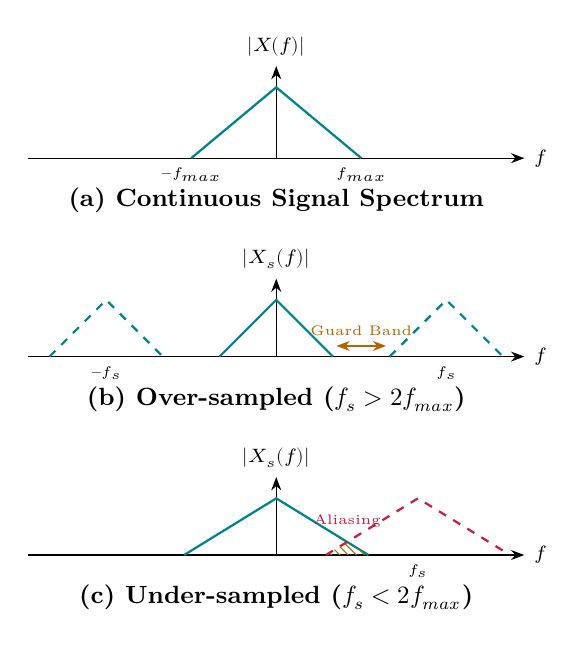
\begin{tikzpicture}[scale=0.9]
  % Axes for (a) Original Spectrum
  \draw[-Stealth, thin] (-3.5, 0) -- (3.5, 0) node[right, font=\scriptsize] {$f$};
  \draw[-Stealth, thin] (0, 0) -- (0, 1.3) node[above, font=\scriptsize] {$|X(f)|$};
  \draw[thick, color=myteal] (-1.2, 0) -- (0, 1.0) -- (1.2, 0);
  \node[below, font=\tiny] at (1.2, 0) {$f_{max}$};
  \node[below, font=\tiny] at (-1.2, 0) {$-f_{max}$};
  \node[font=\small\bfseries] at (0, -0.6) {(a) Continuous Signal Spectrum};

  % Axes for (b) Sampled Spectrum (No Aliasing)
  \begin{scope}[yshift=-2.8cm]
    \draw[-Stealth, thin] (-3.5, 0) -- (3.5, 0) node[right, font=\scriptsize] {$f$};
    \draw[-Stealth, thin] (0, 0) -- (0, 1.1) node[above, font=\scriptsize] {$|X_s(f)|$};
    % Center
    \draw[thick, color=myteal] (-0.8, 0) -- (0, 0.8) -- (0.8, 0);
    % Right replica
    \draw[thick, color=myteal, dashed] (1.6, 0) -- (2.4, 0.8) -- (3.2, 0);
    \node[below, font=\tiny] at (2.4, 0) {$f_s$};
    % Left replica
    \draw[thick, color=myteal, dashed] (-3.2, 0) -- (-2.4, 0.8) -- (-1.6, 0);
    \node[below, font=\tiny] at (-2.4, 0) {$-f_s$};
    % Guard band
    \draw[Stealth-Stealth, thin, color=myamber] (0.85, 0.15) -- (1.55, 0.15);
    \node[above, font=\tiny\color{myamber}] at (1.2, 0.15) {Guard Band};
    \node[font=\small\bfseries] at (0, -0.6) {(b) Over-sampled ($f_s > 2f_{max}$)};
  \end{scope}

  % Axes for (c) Aliased Spectrum
  \begin{scope}[yshift=-5.6cm]
    \draw[-Stealth, thin] (-3.5, 0) -- (3.5, 0) node[right, font=\scriptsize] {$f$};
    \draw[-Stealth, thin] (0, 0) -- (0, 1.1) node[above, font=\scriptsize] {$|X_s(f)|$};
    % Center
    \draw[thick, color=myteal] (-1.3, 0) -- (0, 0.8) -- (1.3, 0);
    % Right replica
    \draw[thick, color=myred, dashed] (0.7, 0) -- (2.0, 0.8) -- (3.3, 0);
    \node[below, font=\tiny] at (2.0, 0) {$f_s$};
    % Overlap region shading
    \fill[pattern=north west lines, pattern color=myamber] (0.7, 0) -- (1.0, 0.18) -- (1.3, 0) -- cycle;
    \node[above, font=\tiny\color{myred}] at (1.0, 0.25) {Aliasing};
    \node[font=\small\bfseries] at (0, -0.6) {(c) Under-sampled ($f_s < 2f_{max}$)};
  \end{scope}
\end{tikzpicture}
\end{tcolorbox}

\subsection{Signal Reconstruction}
Reconstruction is the process of converting discrete samples back into a continuous-time signal. Mathematically, this is done by passing the impulse train through an ideal low-pass filter (cutoff $f_c = f_s/2$). In time domain, this corresponds to the Whittaker-Shannon interpolation formula:
\[
x_a(t) = \sum_{n=-\infty}^{\infty} x(n) \text{sinc}\left(\frac{t - nT_s}{T_s}\right)
\]
In practice, a non-ideal \textbf{Zero-Order Hold (ZOH)} is used, which introduces a frequency roll-off governed by the $\text{sinc}(f/f_s)$ function, requiring a post-reconstruction smoothing filter.

% ===============================================================================
\section{Analog Continuous-Time Filters}
% ===============================================================================

\begin{tcolorbox}[defbox, title={\textbf{Butterworth vs. Chebyshev Filters}}]
\begin{itemize}[leftmargin=*, itemsep=2pt, topsep=0pt]
  \item \textbf{Butterworth Filter:} Characterized by a \textbf{maximally flat} magnitude response in the passband. The transfer function has only poles (no zeros). The magnitude squared is $|H(j\omega)|^2 = 1 / [1 + (\omega/\omega_c)^{2N}]$.
  \item \textbf{Chebyshev Filter (Type I):} Permits \textbf{equiripple behavior} in the passband to achieve a sharper transition band (faster roll-off) for the same filter order $N$.
\end{itemize}
\end{tcolorbox}

\subsection{Passive RC and RL Filters}
A passive filter uses only resistors, capacitors, and inductors. No power supply is needed, but no gain is possible. Passive filters are commonly used as anti-aliasing front-ends before ADC inputs.

\begin{tcolorbox}[formulabox, title={\textbf{First-Order Passive Filter Transfer Functions}}]
\textbf{RC Low-Pass Filter} (series $R$, shunt $C$):
\[
H_{LP}(s) = \frac{1/sC}{R + 1/sC} = \frac{\omega_c}{s + \omega_c} \qquad \omega_c = \frac{1}{RC}
\]
\textbf{RC High-Pass Filter} (series $C$, shunt $R$):
\[
H_{HP}(s) = \frac{R}{R + 1/sC} = \frac{s}{s + \omega_c}
\]
\textbf{RL Low-Pass Filter} (series $R$, shunt $L$):
\[
H_{LP}(s) = \frac{sL}{R + sL} \rightarrow \frac{\omega_c}{s + \omega_c} \qquad \omega_c = \frac{R}{L}
\]
Roll-off rate: $-20\,$dB/decade per filter order. At $\omega = \omega_c$: $|H| = 1/\sqrt{2}$ ($-3\,$dB point).
\end{tcolorbox}

\textbf{Limitations of Passive Filters:}
\begin{itemize}[leftmargin=*, itemsep=2pt]
  \item \textbf{Insertion Loss:} Even in the passband, passive filters attenuate the signal (no gain possible).
  \item \textbf{Loading Effect:} Connecting a load changes the effective cutoff frequency unless a buffer is added.
  \item \textbf{Slow Roll-off:} Only $-20\,$dB/decade per order; higher-order cascaded passive stages are impractical.
\end{itemize}
Active filters (Sallen-Key, Tow-Thomas) solve these limitations using op-amps for isolation and gain.

\subsection{Sallen-Key Active Biquad Filter}
The Sallen-Key is a popular second-order active filter stage (biquad). It uses a single operational amplifier configured as a voltage follower (gain $K \ge 1$) and two RC sections.

\begin{tcolorbox}[tikzbox, title={Second-Order Sallen-Key Low-Pass Active Filter}]
\centering
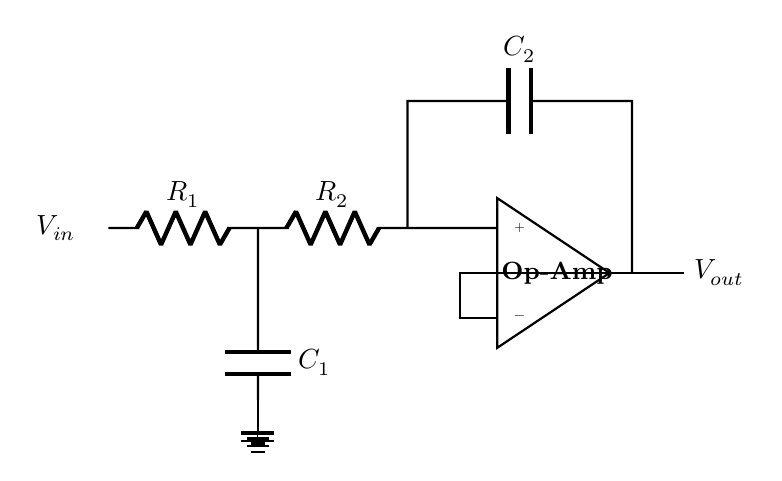
\begin{tikzpicture}[scale=0.95]
  % Op-amp
  \draw[thick] (4, 0.5) -- (4, -1.5) -- (5.5, -0.5) -- cycle;
  \node[font=\tiny] at (4.3, 0.1) {$+$};
  \node[font=\tiny] at (4.3, -1.1) {$-$};
  \node[font=\small\bfseries] at (4.8, -0.5) {Op-Amp};
  \draw[thick] (5.5, -0.5) -- (6.5, -0.5) node[right] {$V_{out}$};

  % Input branch
  \node[left] at (-1.5, 0.1) {$V_{in}$};
  \draw[thick] (-1.2, 0.1) to[R, l=$R_1$] (0.8, 0.1) to[R, l=$R_2$] (2.8, 0.1) -- (4.0, 0.1);
  \draw[thick] (0.8, 0.1) -- (0.8, -1.2) to[C, l=$C_1$] (0.8, -2.2) node[ground] {};
  \draw[thick] (2.8, 0.1) -- (2.8, 1.8) to[C, l=$C_2$] (5.8, 1.8) -- (5.8, -0.5);

  % Feedback and follower gain loop
  \draw[thick] (4.0, -1.1) -- (3.5, -1.1) -- (3.5, -0.5) -- (5.8, -0.5);
  \node[ground] at (0.8, -2.3) {};
\end{tikzpicture}
\end{tcolorbox}

For the Sallen-Key low-pass filter with $R_1 = R_2 = R$ and $C_1 = C_2 = C$ and unity amplifier gain ($K=1$):
\begin{tcolorbox}[formulabox, title={\textbf{Sallen-Key Transfer Function and Parameters}}]
\[
H(s) = \frac{V_{out}(s)}{V_{in}(s)} = \frac{1}{s^2 R^2 C^2 + 2sRC + 1}
\]
Comparing with the standard second-order biquad form $H(s) = \frac{\omega_0^2}{s^2 + \frac{\omega_0}{Q}s + \omega_0^2}$:
\[
\omega_0 = \frac{1}{RC} \qquad \text{(resonant angular frequency)}
\]
\[
Q = \frac{1}{2} = 0.5 \qquad \text{(quality factor)}
\]
\end{tcolorbox}

\subsection{Tow-Thomas State-Variable Biquad Filter}
The Tow-Thomas biquad is a multi-op-amp active filter that is highly stable and easily tunable. It consists of an input summing integrator, a second integrator, and an inverting amplifier to complete the feedback loop.

The transfer function for the Tow-Thomas bandpass output is:
\[
H_{BP}(s) = -\frac{s \frac{1}{R_4 C_1}}{s^2 + s \frac{1}{R_1 C_1} + \frac{1}{R_2 R_3 C_1 C_2}}
\]
This topology allows independent tuning of the gain, frequency $\omega_0$, and quality factor $Q$.

\subsection{Active Gm-C Filters}
At high frequencies (where op-amp open-loop gain drops), active RC filters suffer. \textbf{Gm-C filters} replace resistors and op-amps with \textbf{Operational Transconductance Amplifiers (OTAs)} (which act as voltage-controlled current sources: $I_{out} = g_m V_{in}$) and capacitors.
\begin{itemize}[leftmargin=*, itemsep=2pt]
  \item \textbf{OTA Integrator:} Output current charges a capacitor: $V_{out} = \frac{I_{out}}{sC} = \frac{g_m}{sC} V_{in}$.
  \item \textbf{High-Frequency Tuning:} The transconductance $g_m$ is electronically tunable by adjusting the OTA bias current, allowing real-time frequency tuning.
\end{itemize}

% ===============================================================================
\section{Basics of Analog Discrete-Time Filters \& Z-Transform}
% ===============================================================================

\begin{tcolorbox}[defbox, title={\textbf{Discrete-Time Filter Definition}}]
A discrete-time filter processes sequence samples $x(n)$ to produce output samples $y(n)$. It is described by a linear constant-coefficient difference equation:
\[
y(n) = \sum_{i=0}^{M} b_i x(n-i) - \sum_{j=1}^{N} a_j y(n-j)
\]
\end{tcolorbox}

\subsection{Z-Transform and ROC}
The Z-transform is the discrete-time equivalent of the Laplace transform. For a sequence $x(n)$, it is defined as:
\[
X(z) = \mathcal{Z}\{x(n)\} = \sum_{n=-\infty}^{\infty} x(n) z^{-n}
\]
where $z = r e^{j\omega}$ is a complex variable. The \textbf{Region of Convergence (ROC)} is the set of values in the $z$-plane for which the summation converges.
\begin{itemize}[leftmargin=*, itemsep=2pt]
  \item \textbf{Causal sequence:} ROC is the exterior of a circle ($|z| > R_{max}$).
  \item \textbf{Stable system:} The ROC must contain the unit circle ($|z| = 1$). This implies all poles of the system transfer function $H(z)$ must lie strictly inside the unit circle ($|poles| < 1$).
\end{itemize}

\subsection{Mapping s-Plane to z-Plane}
To design discrete-time filters from continuous-time templates, the s-plane must be mapped to the z-plane.
\begin{enumerate}[label=\textbf{\arabic*.}, leftmargin=*, itemsep=3pt]
  \item \textbf{Impulse Invariance:} Preserves the impulse response shape. The mapping is $z = e^{sT_s}$. This suffers from severe spectral aliasing.
  \item \textbf{Bilinear Transformation (BLT):} Maps the entire left half of the s-plane to the inside of the unit circle in the z-plane. It is defined by the algebraic mapping:
  \[
  s = \frac{2}{T_s} \frac{z - 1}{z + 1} \quad \Rightarrow \quad z = \frac{1 + s T_s/2}{1 - s T_s/2}
  \]
\end{enumerate}

\subsection{Frequency Warping Effect}
The BLT maps the infinite continuous frequency axis $-\infty < \Omega < \infty$ non-linearly to the finite discrete frequency axis $-\pi/T_s < \omega < \pi/T_s$. Substituting $s = j\Omega$ and $z = e^{j\omega T_s}$ gives the frequency relation:
\begin{tcolorbox}[formulabox, title={\textbf{Frequency Warping and Pre-warping Relations}}]
\[
\Omega = \frac{2}{T_s} \tan\left(\frac{\omega T_s}{2}\right)
\]
To compensate for this non-linear compression (warping), continuous-time specifications must be \textbf{pre-warped} before applying the BLT:
\[
\Omega_{pre} = \frac{2}{T_s} \tan\left(\frac{\omega_{desired} T_s}{2}\right)
\]
\end{tcolorbox}

\begin{tcolorbox}[examplebox, title={\textbf{Worked Example: Bilinear Transformation with Pre-warping}}]
\textbf{Problem:} Design a discrete low-pass filter with cutoff $f_d = 2\,$kHz at sampling rate $f_s = 10\,$kHz. Use a first-order continuous-time prototype $H(s) = \frac{\Omega_c}{s + \Omega_c}$.

\textbf{Solution:}
\begin{enumerate}[label=\textbf{\alph*.}, leftmargin=*, itemsep=2pt]
  \item Calculate $T_s = 1/f_s = 10^{-4}\,$s.
  \item Discrete angular frequency $\omega_d = 2\pi f_d = 4000\pi\,\text{rad/s}$.
  \item Pre-warped continuous frequency $\Omega_c$:
    \[
    \Omega_c = \frac{2}{10^{-4}} \tan\left(\frac{4000\pi \times 10^{-4}}{2}\right) = 20000 \tan(0.2\pi) \approx 20000 \times 0.7265 = 14530\,\text{rad/s}
    \]
  \item Apply Bilinear Transformation:
    \[
    H(z) = \left. \frac{\Omega_c}{s + \Omega_c} \right|_{s = \frac{2}{T_s}\frac{z-1}{z+1}} = \frac{14530}{\frac{2}{10^{-4}}\frac{z-1}{z+1} + 14530} = \frac{14530(z+1)}{20000(z-1) + 14530(z+1)}
    \]
    \[
    H(z) \approx \frac{14530(z+1)}{34530 z - 5470} \approx \frac{0.42(z+1)}{z - 0.158}
    \]
\end{enumerate}
\end{tcolorbox}

% ===============================================================================
% QUICK REVISION PAGE
% ===============================================================================
\newpage
\begin{center}
  {\large\bfseries\color{myred} Quick Revision --- Module 1}\\[3pt]
  {\small\color{mydark} Filter Fundamentals and Z-Transform $|$ PE-EC802A}
\end{center}
\noindent{\color{myred}\rule{\linewidth}{1.2pt}}
\vspace{4pt}

\begin{tcolorbox}[formulabox, title={\textbf{Key Formulas and Transforms at a Glance}}]
\renewcommand{\arraystretch}{1.35}
\begin{tabularx}{\linewidth}{B{5.0cm} X}
Nyquist Sampling Rate & $f_s \ge 2 f_{max}$ \\[4pt]
Sinc Reconstruction & $x_a(t) = \sum x(n) \text{sinc}\left(\frac{t - nT_s}{T_s}\right)$ \\[4pt]
Sallen-Key LP frequency & $\omega_0 = \frac{1}{\sqrt{R_1 R_2 C_1 C_2}}$; \quad $Q = \frac{\sqrt{R_1 R_2 C_1 C_2}}{R_1 C_2 + R_2 C_2 + (1-K)R_1 C_1}$ \\[4pt]
Bilinear Transformation & $s = \frac{2}{T_s} \frac{z-1}{z+1}$ \\[4pt]
Frequency Warping relation & $\Omega = \frac{2}{T_s} \tan\left(\frac{\omega T_s}{2}\right)$ \\[4pt]
Z-transform & $X(z) = \sum_{n=-\infty}^{\infty} x(n) z^{-n}$ \\[4pt]
Unit circle frequency map & $z = e^{j\omega T_s}$ \\[4pt]
\end{tabularx}
\end{tcolorbox}

\begin{tcolorbox}[defbox, title={\textbf{One-Line Definitions}}]
\begin{itemize}[leftmargin=*, itemsep=2pt, topsep=0pt]
  \item \textbf{Aliasing:} High frequencies folding back to lower bands due to under-sampling ($f_s < 2f_{max}$).
  \item \textbf{Anti-Aliasing Filter:} A low-pass filter limiting analog signal bandwidth to $f_s/2$ before sampling.
  \item \textbf{Butterworth Response:} Maximally flat magnitude profile in the passband.
  \item \textbf{Chebyshev Response:} Passband equiripple profile resulting in a sharper cutoff transition band.
  \item \textbf{Biquad Filter:} A second-order active filter block implementing a pair of poles and optionally zeros.
  \item \textbf{Gm-C Filter:} A high-frequency filter using transconductance amplifiers and capacitors.
  \item \textbf{ROC:} The region in the z-plane where the Z-transform power series converges.
  \item \textbf{Frequency Warping:} Nonlinear compression of the continuous frequency axis introduced by the bilinear transformation.
\end{itemize}
\end{tcolorbox}

\begin{tcolorbox}[tikzbox, title={\textbf{Analog Filter Topology Comparison}}]
\centering
\par\noindent
\renewcommand{\arraystretch}{1.3}
\begin{tabularx}{\linewidth}{|B{2.6cm}|Y|Y|Y|}
\hline
\textbf{Type} & \textbf{Active Elements} & \textbf{Key Property} & \textbf{Use Case} \\ \hline
\textbf{Passive RC/RL} & None & No gain, simple & AAF, RF matching \\ \hline
\textbf{Butterworth} & Op-amp & Maximally flat passband & General purpose LP \\ \hline
\textbf{Chebyshev} & Op-amp & Equiripple, sharp cutoff & Steeper rolloff needed \\ \hline
\textbf{Sallen-Key} & 1 op-amp & 2nd-order, easy design & Active LP/HP/BP \\ \hline
\textbf{Tow-Thomas} & 3 op-amps & Tunable $\omega_0$, $Q$ & Precision biquad \\ \hline
\textbf{Gm-C} & OTA (no R) & High-freq, tunable & $>100\,$MHz filters \\ \hline
\end{tabularx}
\end{tcolorbox}

\begin{tcolorbox}[exambox, title={\textbf{Frequently Asked / Viva Questions}}]
\begin{enumerate}[topsep=0pt, label=\textbf{Q\arabic*.}, itemsep=5pt]
  \item \Q{State the sampling theorem. What happens if the sampling rate is below the Nyquist rate?}
    The sampling theorem states that the sampling rate $f_s$ must be at least twice the maximum signal frequency component ($f_s \ge 2 f_{max}$). Under-sampling causes high frequencies to overlap with low frequencies, creating irreversible aliasing distortion.
  \item \Q{What is the function of the anti-aliasing filter?}
    It is an analog low-pass filter placed before the sampler to block all frequency components above $f_s/2$, ensuring the sampling condition is satisfied.
  \item \Q{Compare Butterworth and Chebyshev filter characteristics.}
    Butterworth filters are maximally flat in the passband but have a slower roll-off. Chebyshev filters have equiripple passband characteristics and a much steeper roll-off transition band.
  \item \Q{Explain the Sallen-Key active filter configuration.}
    It is a second-order active filter structure using one operational amplifier configured as a voltage follower, providing high input impedance, low output impedance, and easily calculable components.
  \item \Q{What are the advantages of Gm-C filters over active RC filters?}
    Gm-C filters do not need operational amplifiers or resistors. They use transconductance amplifiers (OTAs) and capacitors, making them suitable for high-frequency operation (up to hundreds of MHz) and electronically tunable.
  \item \Q{Why does the bilinear transformation map the left half of the s-plane to the inside of the z-plane unit circle?}
    The BLT maps $s = \sigma + j\Omega$ using $z = (1+sT/2)/(1-sT/2)$. For $\sigma < 0$ (LHP), the numerator magnitude is smaller than the denominator magnitude, ensuring $|z| < 1$ (inside the unit circle).
  \item \Q{What is frequency warping in the Bilinear Transformation, and how is it compensated?}
    It is the non-linear compression of the continuous frequency axis $\Omega$ to the discrete axis $\omega$. It is compensated by pre-warping continuous-time critical frequencies: $\Omega_c = \frac{2}{T_s}\tan(\omega_d T_s /2)$.
  \item \Q{State the condition for a discrete-time LTI system to be stable.}
    The system is stable if its Z-transform region of convergence (ROC) contains the unit circle ($|z|=1$), which requires all poles to lie strictly inside the unit circle.
  \item \Q{What is the Z-transform of a causal sequence $a^n u(n)$? State its ROC.}
    The Z-transform is $H(z) = \frac{z}{z-a}$ (or $\frac{1}{1-a z^{-1}}$) with the region of convergence $|z| > |a|$.
  \item \Q{Why is the impulse invariance mapping not suitable for high-pass and band-stop filters?}
    Impulse invariance maps frequencies linearly, which causes severe aliasing at high frequencies. High-pass and band-stop filters have infinite high-frequency energy, making aliasing unacceptable.
\end{enumerate}
\end{tcolorbox}

\end{document}
